\section{g4tools}
It must be mentionned that good part of the analysis and graphics
technology is shared with Geant4 through the "g4tools" library.


Note that the development repository is still private, mainly because
there is only one active developer for EsbRootView itself.

Today it is based on a detector and event models not shared with the
``batch'' programs done with the EsbRoot framework. If the ESSnuSB projet is continued, it would be a nice
mid/long time target to have these in common with the
batch.

For portability reason EsbRootView is not built over the
EsbRoot framework developed and used for the ESSnuSB simulations.

Alas, the today HEP frameworks, including EsbRoot (based on FairRoot), do not provide
highly portable event and detector models needed to build
event displays able to exploit natively graphics capabilities of
devices we have in hands today.

Anyway, doing EsbRootView is possible due to the fact that we can read ROOT
files, by using our inlib/rroot classes, describing geometries and also events produced by the
simulations based over EsbRoot, and this without the need to tie to
FairRoot and then CERN ROOT. The reading of ROOT files ``without ROOT'' is here the key point that
permits to work.


For an event, we had implemented our own classes (EsbMCTrack,
EsbDetectorPoint, EsbHit, EsbFgdHit) and a one\_event class to keep in
memory vector of instances of these, read from an event file with our
ROOT/IO library.


Obviously
this duplicates the event model classes done in the EsbRoot framework,
but today (2020) the forseen detector descriptions (neard, fard, fgd) are not too
complicated to be able to do that. (Obviously, this way would be not
practicable
if attempting to do a display with the same technology, but on a much
more
complicated existing detector as the ones on the LHC). Being able to
have a common, highly portable, detector and event models shared with
``the batch'' would be highly desirable if going toward more
complicate geometries in the future of ESSnuSB.

For portability reason EsbRootView is not built over the
EsbRoot framework developed and used for the ESSnuSB simulations.

Alas, the today HEP frameworks, including EsbRoot (based on FairRoot), do not provide
highly portable event and detector models needed to build
event displays able to exploit natively graphics capabilities of
devices we have in hands today.

Anyway, doing EsbRootView is possible due to the fact that we can read ROOT
files, by using our inlib/rroot classes, describing geometries and also events produced by the
simulations based over EsbRoot, and this without the need to tie to
FairRoot and then CERN ROOT. The reading of ROOT files ``without ROOT'' is here the key point that
permits to work.

on all these devices (something
that would not be poissble if using CERN ROOT itself).

What we can do to push in this
direction is to improve EsbRootView to go also toward an analysis
tool (we have all the parts to do that), but also to show that our
event model could be connected to a Geant4 simulation. We do not want
to do that alone to superseed what is done around the EsbRoot
framework, but just to show that it is possible to have the hand on
ALL the today technologies (and not only on technologies around the
``batch''), and this by using common event and detector models but also a common
IO service.

\cite{CERN-ROOT}
\bibitem{CERN-ROOT} http://root.cern.ch

Rene Brun and Fons Rademakers, ROOT - An Object Oriented Data Analysis Framework,
Proceedings AIHENP'96 Workshop, Lausanne, Sep. 1996,
Nucl. Inst. & Meth. in Phys. Res. A 389 (1997) 81-86.


\begin{figure}[h]
\centering
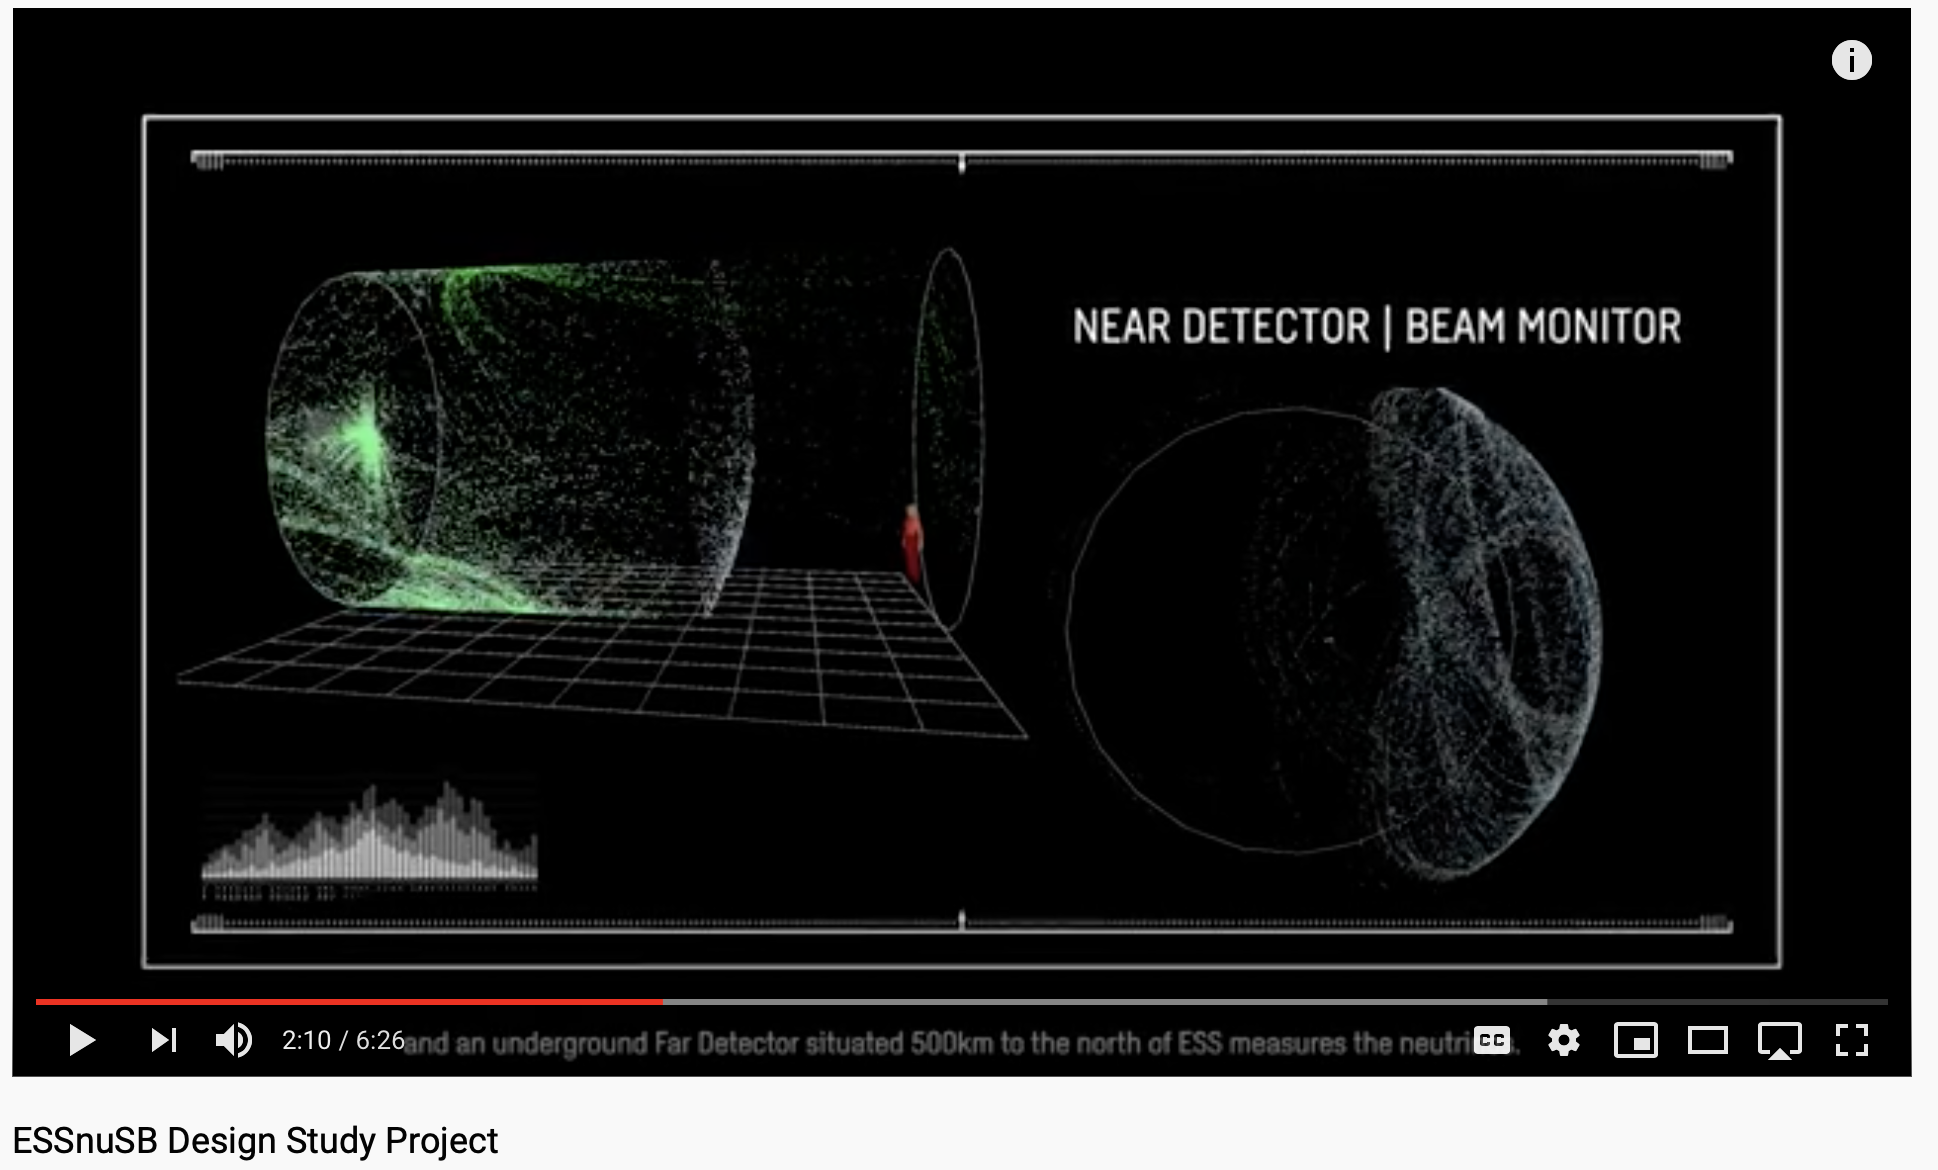
\includegraphics[width=10cm,clip]{youtube_neard}
\caption{Cherenkov light deployment in the neard}
\label{fig-youtube-neard}
\end{figure}

\begin{figure}[ht]
\centering
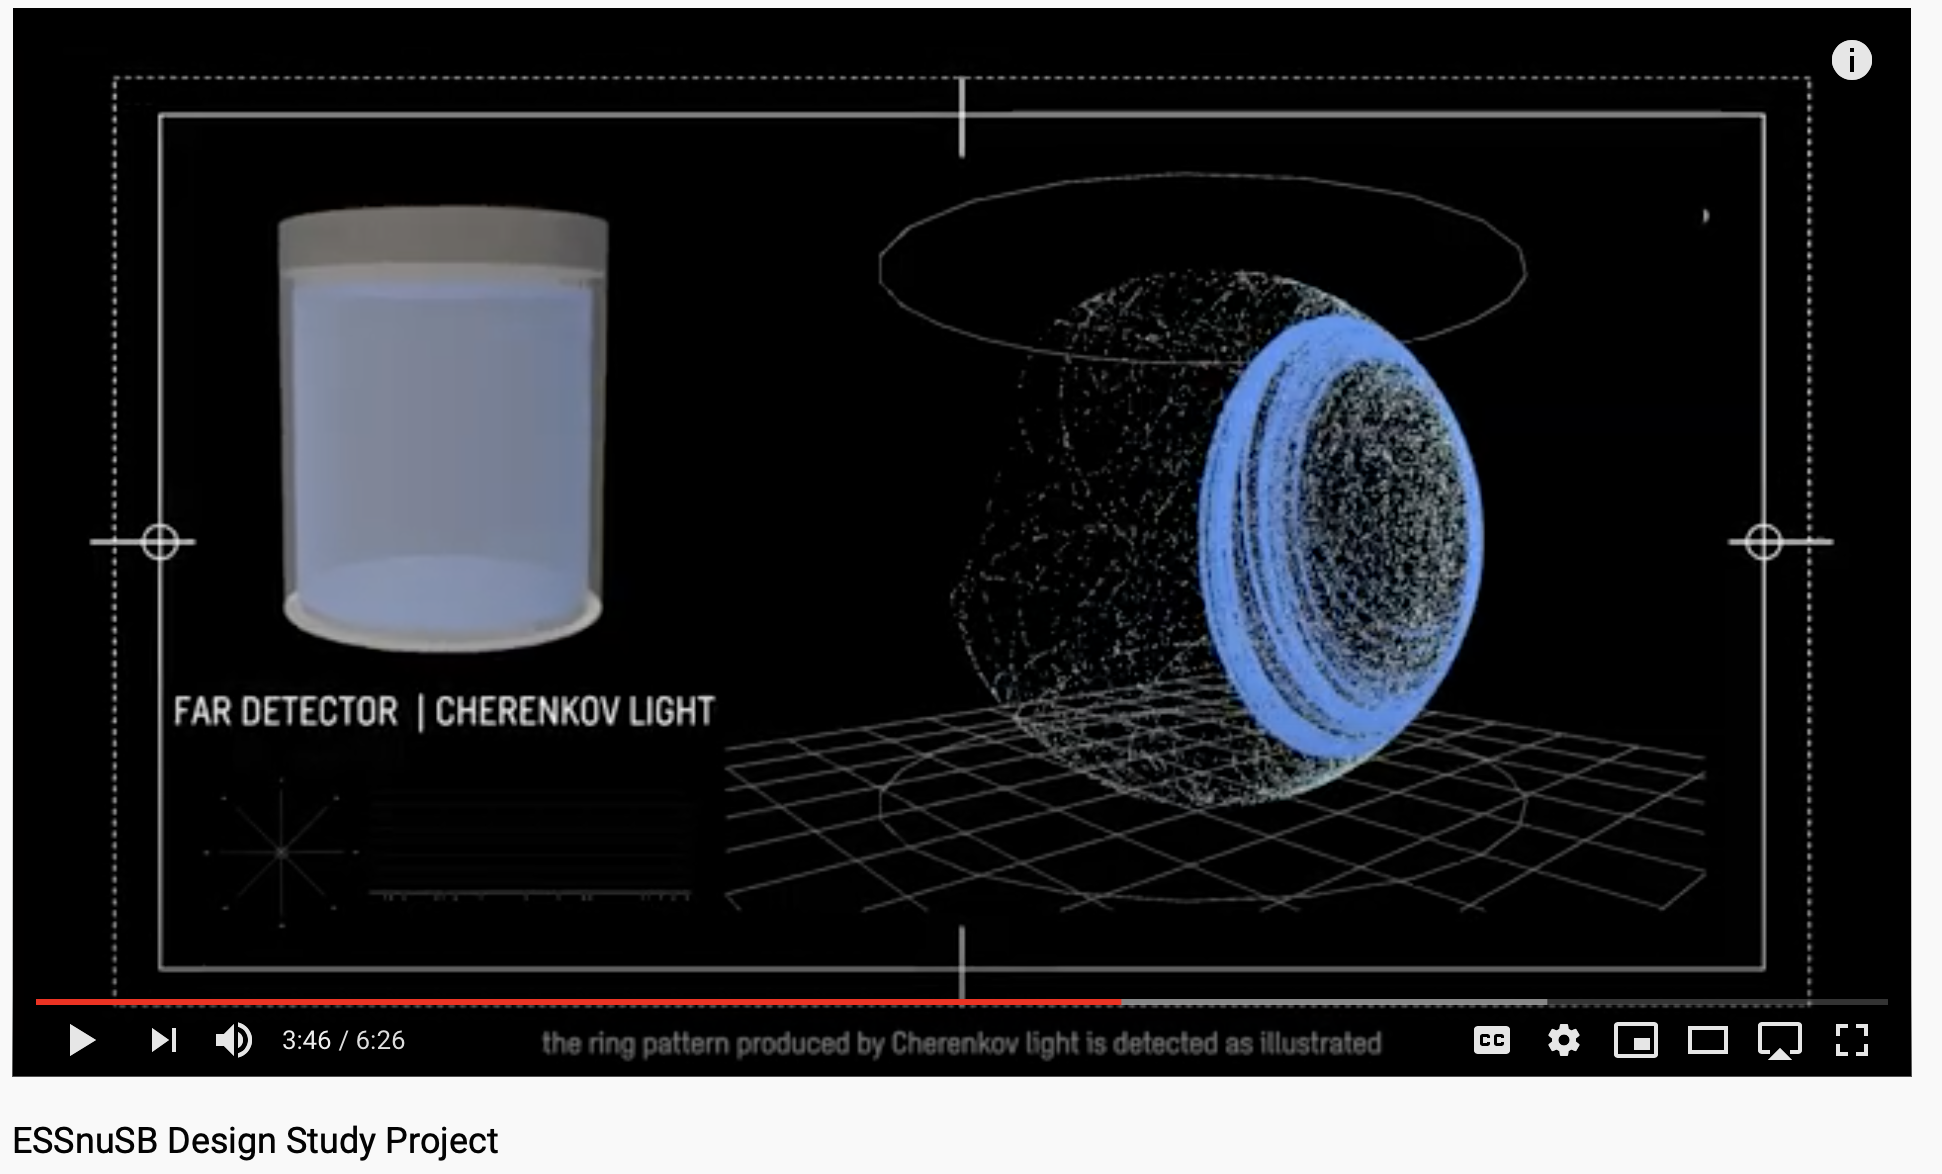
\includegraphics[width=10cm,clip]{youtube_fard}
\caption{Cherenkov light deployment in the fard.}
\label{fig-youtube-fard}
\end{figure}

\begin{figure}[ht]
\centering
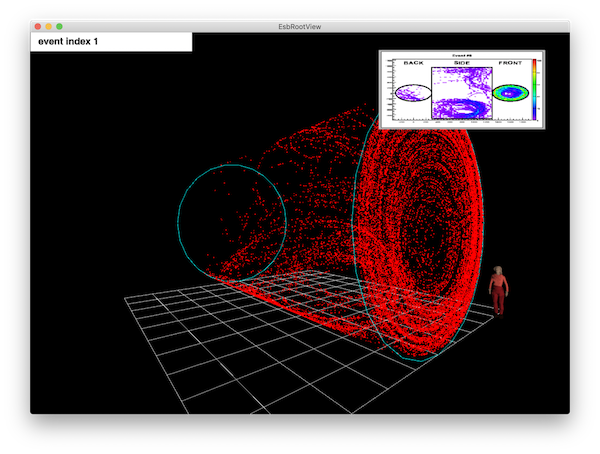
\includegraphics[width=10cm,clip]{layout_event_1}
\caption{DetectorPoint instances in the neard.}
\label{fig-layout-event-1}
\end{figure}

\begin{figure}[ht]
\centering
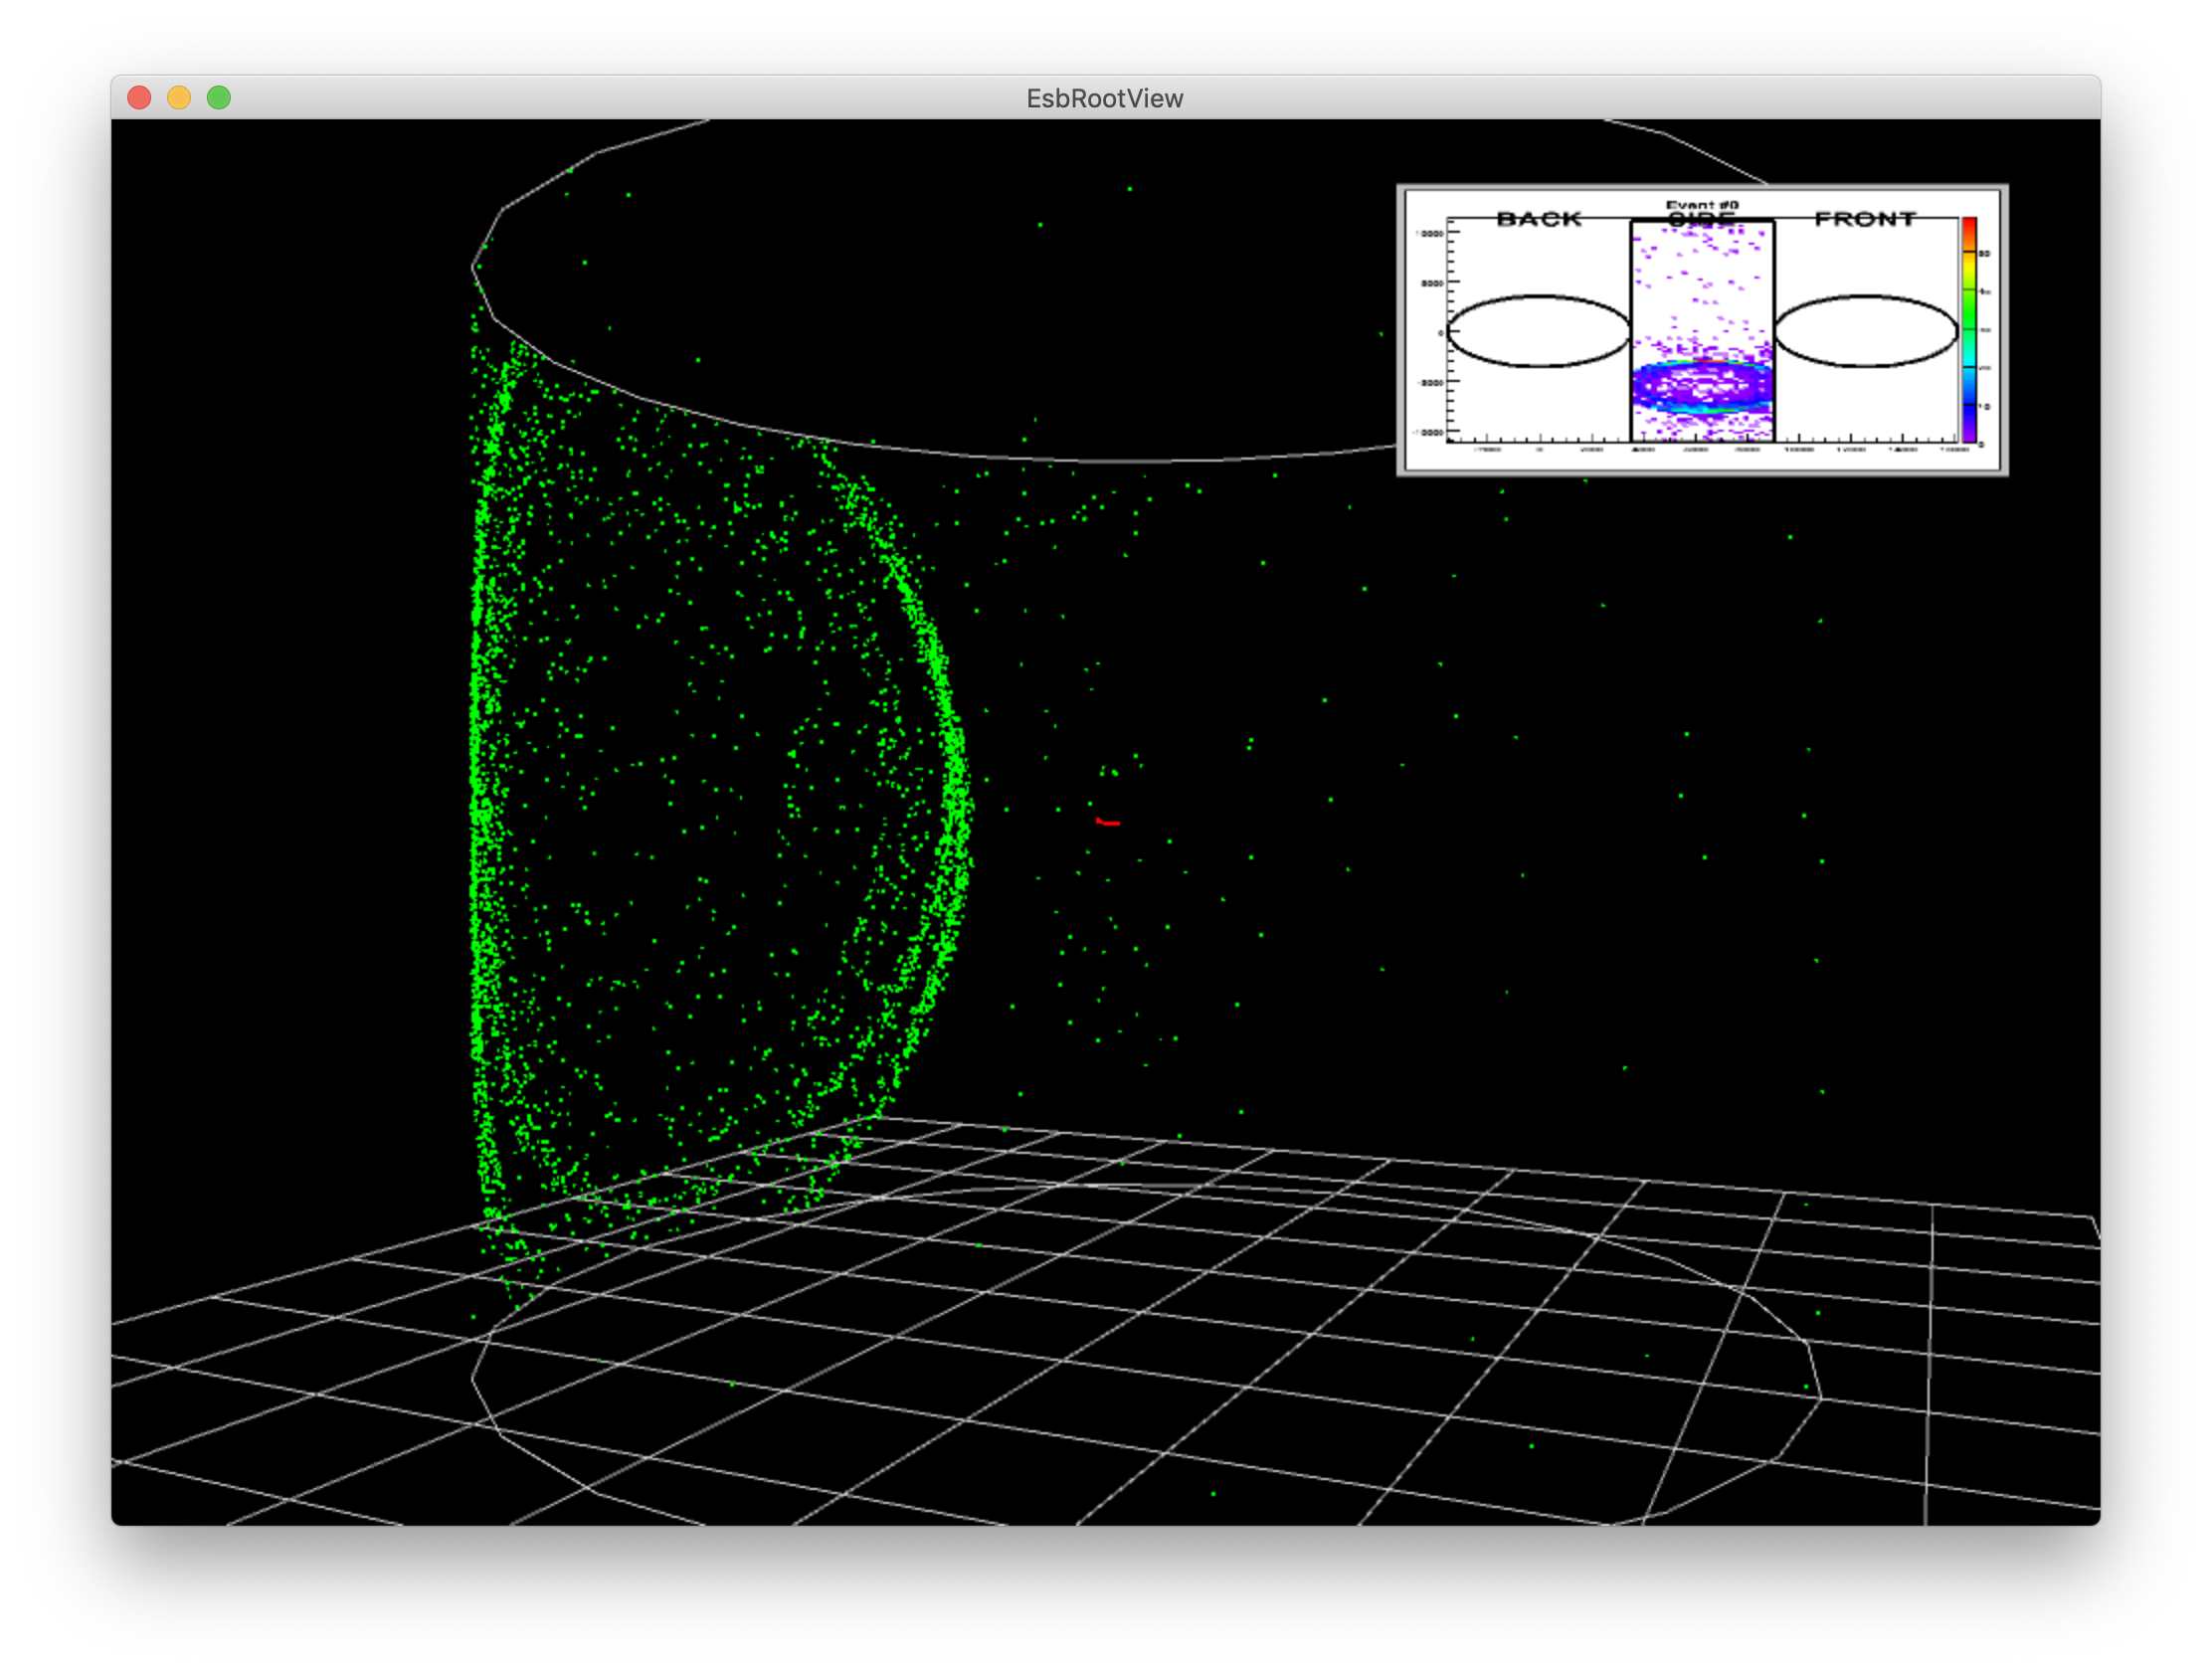
\includegraphics[width=10cm,clip]{fard_setup}
\caption{DetectorPoint instances in the fard.}
\label{fig-fard-setup}
\end{figure}

\begin{figure}[ht]
\centering
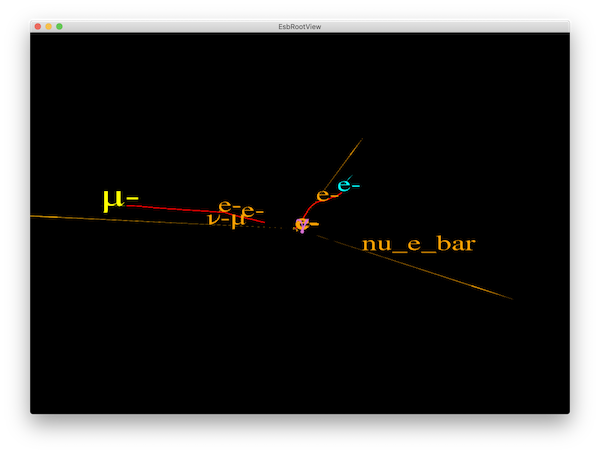
\includegraphics[width=10cm,clip]{neard_MCTrack_arrow}
\caption{A muon decay topology.}
\label{fig-muon-decay}
\end{figure}
